\documentclass{MScthesisITEM}

% this package is just to generate text for demo-purposes
\usepackage{blindtext}
\usepackage{graphicx}
%\graphicspath{/figs}
%\graphicspath{ {/home/sindre/Documents/Master/MasterThesis/Latex/figs} }


\title{Understanding Data Analysis in an\newlinetitle End-to-End IoT System} % The title of your assignement; NB use \newlinetitle to start a newline
\author{Sindre Schei} % Your firstname and lastname
\professor{Frank Alexander Kraemer, ITEM} % Affiliation = ITEM for instance
\supervisor{David Palma, ITEM}

%% Uncomment the following in case you want subfigures; note that there will be a warning for the caption package
% \let\subcaption\undefined
% \let\subfloat\undefined
% \usepackage[bf]{caption}
% \usepackage{subcaption}

\DeclareGraphicsExtensions{.pdf,.jpg,.png}
%\graphicspath{{./figs/}}

\loadglsentries{glossary} 
\makeglossaries

\begin{document}
\selectlanguage{english}
\pagenumbering{roman}
\pagestyle{plain}

%% Only for the project; comment out the line below for the master's thesis; the front page will be generated automatically by DAIM
\titleITEM

%% Only for the master's thesis; for the project report the description is taken from It's Learning and added by the department
% \selectlanguage{english} % Change to 'norsk' if you are writing in Norwegian
% \begin{titlingpage}

\noindent
\begin{tabular}{@{}p{4cm}l}
\textbf{Title:} 	& Understanding Data Analysis in an \\& End-to-End IoT System\\
\textbf{Student:}	& \theauthor \\
\end{tabular}

\vspace{4ex}
\noindent\textbf{Problem description:}
\vspace{2ex}

\noindent The Internet of Things (IoT) is known as the concept of connecting everyday physical devices to the Internet. It is natural to assume that the popularity and development within this field will increase in the following years. This means that more and more things will be able to communicate over the Internet. In the process of developing IoT, an important part is to build reliable and scalable networks, and understanding where data should be processed concerning power consumptions and costs of transferring data in different parts of the network. 

\noindent The task of the thesis will be to access data in a complete prototype of an IoT network, and both collect and analyse the data. The goal is to study different alternatives for a typical IoT system and provide an overview of current state-of-the-art technologies, products and standards that can be used in such a setting. Data can be generated by using and comparing different sensors connected to end nodes in the network.

\noindent To achieve these goals, a central part will be to understand the benefits of processing data in the end nodes, concerning power, costs and time. This means much less data needs to be sent through the network. If the calculations needed are too complex, the measured data needs to be transferred to a central node with higher processing power and easier access of energy. Another part is testing devices and sensors needed, and write programming code associated with these. 

\vspace{6ex}

\noindent
\begin{tabular}{@{}p{4cm}l}
\textbf{Responsible professor:} 	& \theprofessor \\
\textbf{Supervisor:}			& \thesupervisor \\
\end{tabular}

\end{titlingpage}
% \cleardoublepage

%% There must be an abstract in English, even though the main text is in Norwegian
\selectlanguage{english}
%\pagestyle{empty}
\begin{abstract}


\noindent The \gls{iot} is known as the concept of connecting everyday physical devices to the Internet. It is natural to assume that the popularity and development within this field will increase in the following years. This means that more and more things will be able to communicate over the Internet. In the process of developing \gls{iot}, an important part is to build reliable and scalable networks, and understanding where data should be processed concerning power consumption and costs of transferring data in different parts of the network.

\noindent The task of the thesis will be to access data in a complete prototype of an \gls{iot} network, and both collect and analyse the data. The goal is to study different alternatives for a typical \gls{iot} system, and provide an overview of current state-of-the-art technologies, products and standards that can be used in such a setting. Data can be generated by using and comparing different sensors connected to end nodes in the network. A complete network of both \glspl{microcontroller} and \glspl{singleBoardComputer} will be built and explained in this thesis. The network will from now on be referred to as \textit{testbed}. 

\noindent \Glspl{microcontroller} as end nodes in an \gls{iot} network will be the central element tested in this thesis. The main focus is to establish a connection between two devices, A and B, and form a network between these that can transport data efficiently. A central point of discussion will be to find transfer protocols and technologies that can be used in such a network. It will be discussed the advantage and disadvantage of sending raw data, rather than doing computation in end nodes. The main focus will be on optimal throughput in the network. To do this, a deep understanding of the benefits of processing data in the end nodes, concerning power, costs and time is needed. 
%If the calculations needed in the network are too complex to be executed in an end node, the measured data needs to be transferred to a central node with higher processing power and easier access of energy. 

\noindent Results from this work include graphs and discussions explaining in which case the different transport protocols suggested are preferred, from tests done in the testbed. These show that different protocols are suited for different usage, and that one of the tested possibilities more stable than the other in the tests presented. Both protocols registered their highest measured \gls{goodput} at approximately 600 bytes/second. Being a quite slow transfer rate, this opened up for another discussion about the possible use cases for future \gls{ble}-based \gls{iot} applications. 

\noindent Keywords: Optimizing payload sizes, fragmentation, maximizing throughput, power usage. 


\end{abstract}
\cleardoublepage

%% Only for the master's thesis; if the main text is in English and you can write Norwegian, there must be an abstract in Norwegian as well.
\selectlanguage{norsk}
\pagestyle{empty}
\renewcommand{\abstractname}{Sammendrag}
\begin{abstract}
\noindent Tingenes Internet, mer kjent under det engelske navnet Internet of Things (IoT), er konseptet der hverdagslige fysiske gjenstander kobles til Internet. Det er naturlig å anta at populariteten og utviklingen rundt dette vil være økende de kommende årene. Dette betyr at flere og flere ting vil kunne kommunisere over Internet. I prosessen der Tingenes Internet utvikles, er en viktig del å bygge pålitelige og skalerbare nettverk, samt å forstå hvor i nettverket data bør prosesseres med tanke på energibruk og kostnader ved å overføre data mellom deler av nettverket. 

\noindent Hovedoppgaven presentert i denne avhandlingen vil være å jobbe med data i en komplett prototype av et Tingenes Internet-nettverk, og både samle og analysere dataene. Målet er å studere de forskjellige alternativene til et slikt nettverk, samt lage en oversikt over teknologiene og standardene som kan bli brukt i denne sammenhengen. Nødvendig data kan samles ved å sammenligne forskjellige sensorer koblet til endenodene i nettverket. Et komplett nettverk bestående av både mikrokontrollere og små datamaskiner på en brikke, vil bli bygget og forklart i denne oppgaven. Dette nettverket vil fra nå av refereres til som \textit{testbed}. 

\noindent Et sentralt testelement i denne oppgaven vil være bruk av mikrokontrollere som endenoder i et Tingene Internet-nettverk. Hovedfokuset er å sette opp en nettverksforbindelse mellom to enheter, A og B, og danne et nettverk mellom disse slik at data kan overføres på en effektiv måte. I diskusjonen vil et viktig punkt være å finne transportprotokoller og teknologier som kan benyttes i et slikt nettverk. Det vil bli diskutert fordelene og ulempene ved å transportere rådata istedenfor å gjøre utregninger i endenodene. Hovedpoenget her vil være gjennomstrømmingen av data i nettverket. For å gjøre dette trengs en dyp forståelse av fordelene ved å prosessere data i endenodene med tanke på energi, kostnader og tid. 

\noindent Resultatene fra arbeidet består av grafer og diskusjoner rundt disse for å forklare i hvilke situasjoner de forskjellige protokollene som har blitt testedt er foretrukket. Utgangspuntket er tester gjort i testbed. Disse testene viser at de forskjellige protokollene egner seg i ulike situasjoner, men at en av de er mer stabil enn den andre protokollen som denne avhandlingen presenterer. Begge protokollene hadde høyest målte \textit{gls{goodput}} på omkring 600 bytes/sekund. Siden dette er en forholdsvis lav sendingsrate åpnet dette for en annen diskusjon om mulig bruk i fremtidige Tingenes Internett-nettverk der lavenergi Bluetooth er benyttet.

\noindent Nøkkelord: Optimalisering av størrelser på faktiske data, fragmentering av datapakker, maksimere pakkegjennomstrømning, energiforbruk. 


  
\end{abstract}
\cleardoublepage

\selectlanguage{english}% Change to 'norsk' if you are writing in Norwegian

\renewcommand{\abstractname}{Preface}
\begin{abstract}

This thesis was issued by the Department of Telematics (ITEM) at the Norwegian University of Science and Technology (NTNU) the spring of 2016 as a Master Thesis in Telematics. 
The responsible professor has been Frank Alexander Kraemer, ITEM, who has given
helpful advice on how to build up and write such a large project, as
well as answering questions and providing support the whole period. David Palma has been the supervisor, giving impressively close monitoring of the project to fill in ideas, thoughts and good advice to help me finish the thesis. I would like to thank both these ITEM representatives for the work they have put down to make this project as good as possible. 

Secondly, I would like to thank fellow students for the many discussions, good advice and other more social activities the last five years. I would like to point out the guys at A-179 for their support, Jon Anders for helping me with code specific problems during the programming period, and Anders for the many hours we spent together setting up central parts of the network described in this thesis. Special thanks to you!

Last, but not least, I would like to thank my family for their support both during the period of this thesis, but also during my entire period as a student. Special thanks to my father, Svenn Arne, for helping me review the thesis and to get a discussion point with someone without a technical background. 



\end{abstract}
\cleardoublepage

% similarly you may add a separate acknowledgments page

\tableofcontents*
\cleardoublepage

%% include if relevant
\listoffigures
\cleardoublepage

%% include if relevant
\listoftables
\cleardoublepage

%% include if relevant
\listofalgorithms
\addcontentsline{toc}{chapter}{List of Algorithms}
\cleardoublepage

%% include if relevant
\printglossary[title=List of Symbols, style=long]
\cleardoublepage
\glsaddall[]

%% include if relevant
\printglossary[title=List of Acronyms,type=\acronymtype] % prints just the list of acronyms
\cleardoublepage

\pagenumbering{arabic}
\pagestyle{ruled}
%\chapter{Example}
\label{chp:example} 

Here is an example of how to use acronyms such as \gls{ntnu}. The second time only \gls{ntnu} is shown and if there were several you would write \glspl{ntnu}. And here is an example\footnote{A footnote} of citation~\cite{Author:year:XYZ}. 

\Blindtext[3][1]

\begin{figure}
\centering
% dummy figure replacement 
\begin{tabular}{@{}c@{}}
\rule{.5\textwidth}{.5\textwidth} \\
\end{tabular}
\caption{\label{fig:example}A figure}
\end{figure}

\section{First section}\label{sec:first_section}

\subsection{First subsection with some \texorpdfstring{$\mathcal{M}ath$}{Math} symbol}\label{sec:first_ssection}

\blindtext
\begin{itemize}[topsep=-1em,parsep=0em,itemsep=0em] % see http://mirror.ctan.org/macros/latex/contrib/enumitem/enumitem.pdf for details about the parameters
 \item item1
 \item item2
 \item ...
\end{itemize}

\subsection{Mathematics}

\blindmathtrue
\blindtext

\begin{proposition}\label{def:a_proposition}
A proposition... (similar environments include: theorem, corrolary, conjecture, lemma)

\end{proposition}

\begin{proof}
\vspace*{-1em} % Adjust the space when parskip is set to 1em
And its proof.
\end{proof}

\begin{table}
\caption{\label{tab:example}A table}
\centering
\begin{tabular}[b]{| c | c | c | c | c |}
\hline
a & b & c & d & e \\ \hline
f & g & h & i & j \\ \hline
k & l & m & n & o \\ \hline
p & q & r & s & t \\ \hline
u & v & w & x & y \\ \hline
z & æ & ø & å &   \\ \hline
\end{tabular} 
\end{table}

\subsection{Source code example}

% \floatname{algorithm}{Source code} % if you want to rename 'Algorithm' to 'Source code'
\begin{algorithm}[h]
  \caption{The Hello World! program in Java.}
  \label{hello_world}
  % alternatively you may use algorithmic, or lstlisting from the listings package
  \begin{verbatim}
  
class HelloWorldApp {
  public static void main(String[] args) {
    //Display the string
    System.out.println("Hello World!");
  }
}
\end{verbatim}
\end{algorithm}

You can refer to figures using the predefined command like \fref{fig:example}, to pages like \pref{fig:example}, to tables like \tref{tab:example}, to chapters like \Cref{chp:example} and to sections like \Sref{sec:first_section} and you may define similar commands to refer to proposition, algorithms etc.

%% include here the other chapters

\chapter{Introduction}
\label{chp:introduction} 


\section{Motivation}

Internet of Things (IoT) 



is known as the concept of connecting everyday physical devices to the Internet. It is natural to assume that the popularity and development within this field will increase in the following years. This means that more and more things will be able to communicate over the Internet. In the process of developing IoT, an important part is to build reliable and scalable networks, and understanding where data should be processed concerning power consumptions and costs of transfering data in different parts of the network.

\section{Methodology}

\section{Scope and Objectives}

\subsection{Scope}

\subsection{Objectives}

\noindent \textbf{O.1: Build a star network of microcontrollers}

\noindent\textbf{O.2: Connect sensors to the end-nodes to collect data}

\noindent\textbf{O.3: Gather information of the data sent through the network}

\noindent\textbf{O.4: Analyse and discuss the gathered information}

\section{Structure}

\chapter{Background}
\label{chp:background} 

This thesis describes the setup and usage of an End-to-End \gls{iot} system. In order for this to be set up by others later to perform reproducible tests, a detailed description of components, sensors and protocols used is needed. This chapter will go through the background information of the devices, technologies and protocols used, and why these where chosen over other alternatives. 

%\section{Internet of Things} % Tjae

%Comment: Read Future Internet: The Internet of Things from 2010.  \cite{gubbi2013internet}

%Comment: Read http://ac.els-cdn.com/S1570870512000674/1-s2.0-S1570870512000674-main.pdf?_tid=6f15526e-eae8-11e5-addc-00000aab0f6b&acdnat=1458072152_0740a71f559cd8ae1ebd0ce4a687e122

%M2M and "M2T" ("Machine to Thing-communication"). Classification of a thing? \cite{tan2010future}. 

%\section{Challenges}


\section{Bluetooth Low Energy (Bluetooth Smart)}

%Read this:

\gls{ble} is a wireless technology for short range communication developed by the Bluetooth Special Interest Group \cite{gomez2012overview}. The idea was to create a low energy single-hop network solution for \glspl{pan}. A major advantage of this is that Bluetooth 4.0 is already a well established technology in cell phones, laptops and several other devices, and \gls{ble} can use several similarities with this. The 6LoWPAN Working Group has recognized the importance if \gls{ble} in \gls{iot} \cite{hui2008extending}.

The protocol stack of \gls{ble} has two main parts, the controller and the host. In the system used in this thesis this represents the Raspberry Pi as the controller (master) and Nordic nRF52 as the host (slave). The communication between these is done through the standard \gls{hci}. All slaves are in sleep mode by default, and are woken up by the master when communication is needed. Links are being identified by a randomly generated 32-bit code. 

In the case of the network used in this thesis, when the \gls{ble} slave has been connected to a master, it stops searching for other masters, and it is not possible to connect to several masters. This means that we are only able to create a \textit{star network}, not a \textit{mesh network}. This could possibly be an idea for improvement later. Other than this, \gls{ble} seems like a very good alternative in this project. 



Check out: Mikhail Galeev - BLE

\subsection{\gls{hci}}

\subsection{ACL}

\section{6LoWPAN}

%To identify sensors and devices in low energy sensor and device networks, a new protocol was needed. 

\gls{6lowpan} is a defined protocol for using \gls{ipv6} in low enerdy networks, to identify sensors and devices, as defined in the IEEE 802.15.4. 

To use the Internet Protocol was proposed by Geoff Mulligan and the 6LoWPAN Working Group in \cite{mulligan20076lowpan}. In this paper the advantage of \gls{6lowpan} is explained as the easiest way to use standard protocols such as \gls{udp}, \gls{tcp}, \gls{icmp}, gls{dns} and \gls{tftp}, since they can be used directly without the requirement of a translation mechanism. They are already adapted to run over \gls{ipv6}. 

In addition to this, the paper argues that \gls{6lowpan} was developed to be used in small sensor networks. Implementations can fit into 32Kb flash memory parts, wich is smaller than Zigbee and Zensys (which is the two main comparisons made in the paper). It also uses an impressive header comparison mechanism that allows the transmission of \gls{ipv6} packets in 4 bytes, much less than the standard 40 bytes. This is done by using stacked headers, same as in the \gls{ipv6} model, rather than defining a specific header as for \gls{ipv4}. This means that a device can send only the required part of the stack header, and does not need to include header fields for networking and fragmentation \cite{hui2008extending}. 

\gls{6lowpan} was therefore a natural tool to use in this project, in the \gls{ipv6} and \gls{ble} based network. 

%The \gls{6lowpan} architecture was developed to allow \gls{ipv6} packets to be sent over low energy networks.  

\section{Raspberry Pi}

Developed by Element 14, the Raspberry Pi has become a central tool for many people wanting to get started using microcomputers. This was therefore a natural starting point for us as well. 

\begin{figure}[ht]
    \centering
    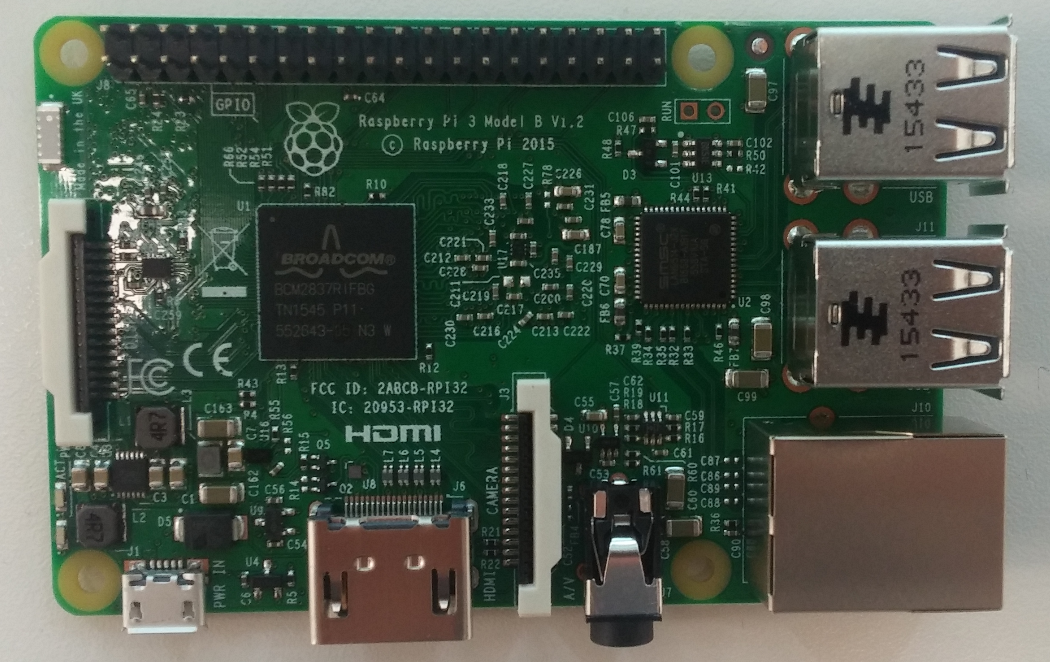
\includegraphics[scale=0.35]{pi3.png}    
    \caption{Raspberry Pi 3}
    \label{fig:piPicture}
\end{figure}



The Raspberry Pi 2 model B+ is the second generation of its kind, and its \textit{ARMv7 processor} has approximately six times the performance of the predecessor \cite{raspberryPi2}. With a USB Bluetooth dongle connected, it is quite simple to enable both \gls{6lowpan} and \gls{ble}, given that the right Unix kernel has been used in the \gls{os} of the Pi.

Later in this thesis, the processing power of the Pi compared to performing calculations in the end-points will be a central topic for discussion. 

\subsection{Ubuntu Mate}

Along with the Raspberry Pi, we needed a good and stable operating system with a kernel that supported the \gls{6lowpan} architecture. For this, Ubuntu Mate version 15.10 with kernel version 4.15 was chosen, and used on the Raspberry Pi. As other versions of Ubuntu this is Unix based, and has a complete \gls{gui} of a full \gls{os}. 

\section{nRF52}

The nRF52 is developed by Nordic Semiconductor, and is being described as a family of highly flexible, multi-protocol system on chip. 

% Kok 

\begin{figure}[ht]
    \centering
    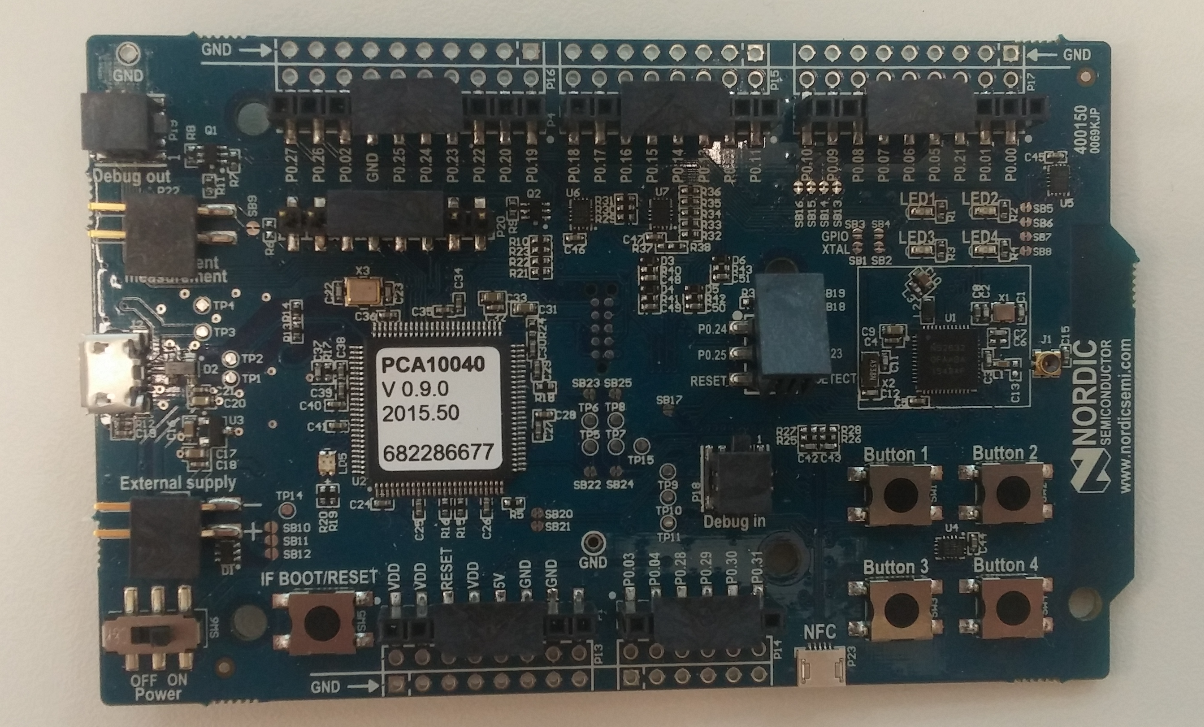
\includegraphics[scale=0.32]{nrf52.png}    
    \caption{Nordic Semiconductor NRF52}
    \label{fig:nrf52picture}
\end{figure}

\cite{nrf52Nordic}

Running at 64MHz it racks up impressive stats: EEMBC Coremark® score of 215 and 58 Coremark®/mA. Built in a cutting edge 55nm process technology the nRF52 Series is architected for todays need for speed, speed to carry out increasingly complex tasks in the shortest possible time and return to sleep, conserving precious battery power. Introducing a Cortex-M4F processor at its heart, it is the most capable Bluetooth Smart SoC on the market today.	
With a brand new multiprotocol radio architecture limits are pushed even further for Bluetooth Smart: A total link budget of 100dBm, -96dBm sensitivity, +4dBm output power and -42dBm selectivity, it is built to exist reliably and effectively in a busy 2.4GHz band. Couple this RF resilience with outstanding power consumption: 5.3mA at 0dBm TX output power and 5.4mA RX it is miserly with power when getting things done on-air.

 

Designed with wealth of digital and analog interfaces and peripherals, there’s something to cover every design requirement. The demands of today’s Bluetooth smart single chip designs are increasingly varied and complex, they can range from digital audio processing, to FFT/FIR and security algorithms, to driving device displays and UIs. Whatever the task, nRF52 series has it covered.

 

We’ve truly made low power easy. We haven’t just just great datasheet numbers, but an automatic and adaptive power management system which combined with extensive EasyDMA and PPI makes the nRF52 Series positively frugal with power.

 

nRF52 Series brings NFC for the first time to a Bluetooth Smart SoC. The on-chip NFC-A tag allows developers to take advantage of NFC ‘touch-to-pair’ functionality in their designs.

 

Maintaining the total flexibility philosophy of the nRF51 Series, it is a flash device. With 512kB flash + 64kB RAM on chip, developers keep all the software stack flexibility and Over-The-Air Device Firmware Upgrade (OTA-DFU) features they enjoyed with the nRF51 Series.

 

We understand that in the world of wearables, size really is everything, so we built a device that is the smallest Bluetooth Smart SoC to date measuring as small as 3.0 x 3.2mm (CSP). With an on-chip balun and a minimum of external components it has the smallest design footprint out there.

 

Tomorrow’s Bluetooth Smart Solutions are going to ask a lot. The nRF52 Series delivers.

% Kok slutt


% https://www.nordicsemi.com/Products/nRF52-Series-SoC

\subsection{Softdevice}




\section{Adafruit ADXL345 Accelerometer}

In order to do collect data, a sensor needed to be connected to the Nordic Semiconductor nRF52. The main thought behind the thesis was to measure vibrations, and a good accelerometer was needed. The Adafruit ADXL345 accelerometer was chosen for several reasons. 

\begin{itemize}
  \item It is the same accelerometer built in on the Zolertia Z1 microcontroller
  \item It can measure acceleration in all three axes, X, Y and Z.
  \item It sends digital data right away. This means there is no need to use computational power to calculate digital values as needed if the data was captured by an analog accelerometer. 
  \item It supports both \gls{i2c} and \gls{spi}, which makes it easy to connect to the nRF52. 
\end{itemize}


\begin{figure}[ht]
    \centering
    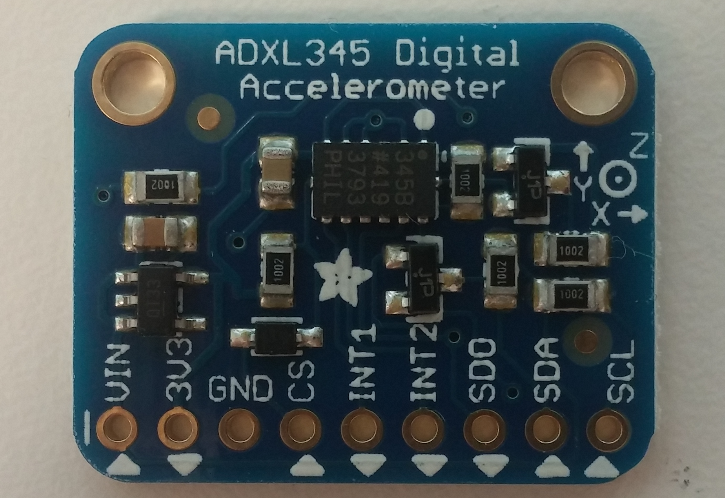
\includegraphics[scale=0.32]{ADXL345.png}    \caption{ADXL345 Accelerometer}
    \label{fig:adxl345}
\end{figure}

\newpage

\section{Transport protocols}

\subsection{Network layers}

\subsection{\gls{coap}}

%The \\ protocol is described in the documentation as follows: 

\gls{coap} is a transport protocol designed to be used in constrained networks for \gls{m2m} communication. It is \gls{udp} based, and works good in low-power and lossy networks. It can be used with microcontrollers, and with \gls{ipv6} and \gls{6lowpan}. Both GET and PUSH functionality can be used, as well as \textit{observable} GET. This means that a server can "subscribe" to end notes in the network, and get updates either after a given timespan or when changes have been made. This therefore looked like a promising protocol to use, and was chosen as the first transport protocol to test the network \cite{shelby2014constrained}.
 



\subsection{\gls{mqtt}}

Another transport protocol that could be used in such a network of microcontrollers is \gls{mqtt}. This is  known as a publish-subscribe based on \gls{tcp}, using a \gls{mqtt} broker. \gls{ntnu} does have a broker that is possible to use, or a broker can be rented from several other places. Here a 

\cite{hunkeler2008mqtt}

\subsection{\gls{radvd}}


\section{Software tools}

As \gls{ide}, the \textit{KEIL Vision} was used, as recommended by Nordic Semiconductor (where?), for writing C programming. For other programming languages (for instance Python 3.4, HTML, CSS, JavaScript, Flask and AJAX) \textit{Sublime Text 2} for Windows and Linux was used, as well as \textit{Pluma} for Ubuntu Mate on the Raspberry Pi. 

\subsection{Other}

Wireshark, Firefox, GitHub







\chapter{System Architecture}
\label{chp:architecture} 

The purpose of this thesis is to build an end-to-end system, to be able to transfer data all the way from sensors connected to a microcontroller to a server. This chapter will describe in detail how the different components of the system has been connected together, and how the different protocols has been configured to read and transfer data efficiently. 


\begin{figure}[ht]
    \centering
    \includegraphics[scale=0.7]{MasterArchitecture2.png}    
    \caption{System architecture}
    \label{fig:systemArchitecture}
\end{figure}

Figure \ref{fig:systemArchitecture} shows how the complete end-to-end system of this thesis is set up. In short terms, the \textit{Nordic Semiconductor nRF52} is connected to a  \textit{Raspberry Pi 3} using \gls{6lowpan} and \gls{ble}. This means that they are able to communicate using \gls{ipv6} addresses, even though the nRF52 only has a bluetooth antenna built in, as shown in figure \ref{fig:nrf52chipDetail}. The limitations of \gls{ble} means that the nRF52 can only connect to \textit{one} device at the time. Several of these put together are therefore forming a \textit{star network} using the \textit{Raspberry Pi} as a central point of connection. Computations can now either be done in the end nodes at the \textit{nRF52s}, at the \textit{Raspberry Pi}, or forwarded to a web server or another computer with more computational power. Data can also be displayed directly to a web page from the \textit{Raspberry Pi}. 
 
%\newpage

There are in general three main limitations in a network such as this:

\renewcommand{\labelitemi}{$\textasteriskcentered$}
\begin{itemize}
  \item Computational power in the different nodes
  \item Battery capacity of the end nodes
  \item Network limitations between the nodes
\end{itemize}

A central part of the testing in this thesis will be to test the different limitations, and to understand the pros and cons of doing computations in end nodes, compared to transferring information to a server with \textit{much} more computational power. Power usage is very often closely related to computational power, and will also be a central factor. The next section will contain a walk-through of the system, from the smallest to the biggest component, to explain their computational and power capabilities, and how they can communicate efficiently. 

Computational power is closely related to power usage. The nRF52 microcontroller is battery powered using a small \textit{3V Lithium CR 2032} battery. Given this limitation the computational power will be limited as well. The optimal solutions therefore seems to handle as little data as possible here. 


\section{Connecting Raspberry Pi and nRF52}


%As a microcontroller the nRF52 works good in this network, both as a low-power and powerful device. 

To set up the communication between a Raspberry Pi and the nRF52, the two code examples TWI and Observable server from Nordic Semiconductor was used as a starting point for coding on the nRF52. It was however quite tricky to set connect these two together the first time. The following recipe is what worked best. 

Install an \gls{os} on the Raspberry Pi that has a Linux kernel version later than 3.18. On \textit{Raspbian} version 3.18 is the only stable (Note: Jan. 2016), but \textit{Ubuntu Mate} is stable in version 4.15. \textit{Ubuntu Mate} was therefore chosen as the best and most stable \gls{os}. When this is done a resizing of the file system is needed to use all the capacity of the memory card. This is not necessary, but recommended to be able to use more than 4GB of the memory card. To resize, run the following commands

\begin{verbatim}
sudo fdisk /dev/mmcblk0
\end{verbatim}

Delete partition (d,2), and run the following after a reboot

\begin{verbatim}
sudo resize2fs /dev/mmcblk0p2
\end{verbatim}

To use \gls{ble}, install Bluez and radvd using \textit{apt-get} in a \textit{Unix terminal}:

\begin{verbatim}
apt-get install radvd wireshark bluez
apt-get upgrade
apt-get update
\end{verbatim}
%\end{lstlisting}

To activate \gls{ipv6} forwarding, uncomment the following line (remove "\#") in the file \textit{etc/sysctl.conf}

\begin{verbatim}
net.ipv6.conf.all.forwarding=1
\end{verbatim}

Add the \textit{bt0 interface} in \textit{radvd.conf}:

\begin{verbatim}
touch /etc/radvd.conf
pico /etc/radvd.conf
\end{verbatim} 

Write in the bt0 interface

\begin{verbatim}
interface bt0
{
    AdvSendAdvert on;
    prefix 2001::/64
    {
        AdvOnLink off;
        AdvAutonomous on;
        AdvRouterAddr on;
    };
};
\end{verbatim} 

To mount the modules \textit{bluetooth\_6lowpan, 6lowpan and radvd}, add the following to \textit{/etc/modules}. 

\begin{verbatim}
bluetooth_6lowpan
6lowpan
radvd
\end{verbatim}

It is now possible to use the \textit{hcitool} command. 

\begin{verbatim}
hcitool lescan
\end{verbatim}

This command will scan for \gls{ble} devices nearby, and find the bluetooth address, for instance \textit{0211:22FF:FE33:4455}. The normal procedure in this case would be to run the following command: 

\begin{verbatim}
echo 1 > /sys/kernel/debug/bluetooth/6lowpan_enable
hcitool lecc 0211:22FF:FE33:4455
service radvd restart
\end{verbatim}

This command never established a stable connection in this system. It was not possible to test the connection, and each connected device became automatically disconnected after about 15 seconds. The reason for this was never found. Instead it was possible to not use \textit{hcitool} for this part, and the following commands worked fine:

\begin{verbatim}
echo 1 > /sys/kernel/debug/bluetooth/6lowpan_enable
echo "connect 0211:22FF:FE33:4455 1" > /sys/kernel/
debug/bluetooth/6lowpan_control
service radvd restart
\end{verbatim} 
\todo{FIX verbatim new line? }

The command \textit{hcitool con} shows the connected \gls{ble} devices. If the device is connected, the connection can be tested by typing:

\begin{verbatim}
ping6 2001::0211:22FF:FE33:4455
\end{verbatim}


Using the basic examples provided by Nordic Semiconductor described in chapter \ref{chp:architecture}.3, it was now possible to send messages both using \gls{coap} \gls{con} and \gls{non}.  


\section{Connecting nRF52 and ADXL345}

\todo{Can possibly write much more here, code samples in appendix, things that needed to be changed and so on}

The ADXL345 Accelerometer used was connected using \gls{i2c}, which is quite straight forward using the nRF52. Connection scheme is as follows (nRF52 -> ADXL345): 

\begin{itemize}
  \item 5V -- VIN		\tab  	\textit{Power source, \textbf{\textcolor{green}{green cable}} in Figure \ref{fig:nrf-adxl345}}
  \item GND -- GND 		\tab 	\textit{Ground, \textbf{\textcolor{red}{red cable}} in Figure \ref{fig:nrf-adxl345}}
  \item P0.27 -- SDA	\tab	\textit{\gls{i2c} Serial Data Line, \textbf{\textcolor{orange}{orange cable}} in Figure \ref{fig:nrf-adxl345}}
  \item P0.26 -- SCL	\tab 	\textit{\gls{i2c} Serial Clock Line, \textbf{\textcolor{brown}{brown cable}} in Figure \ref{fig:nrf-adxl345}}
\end{itemize} 

\begin{figure}[ht]
    \centering
    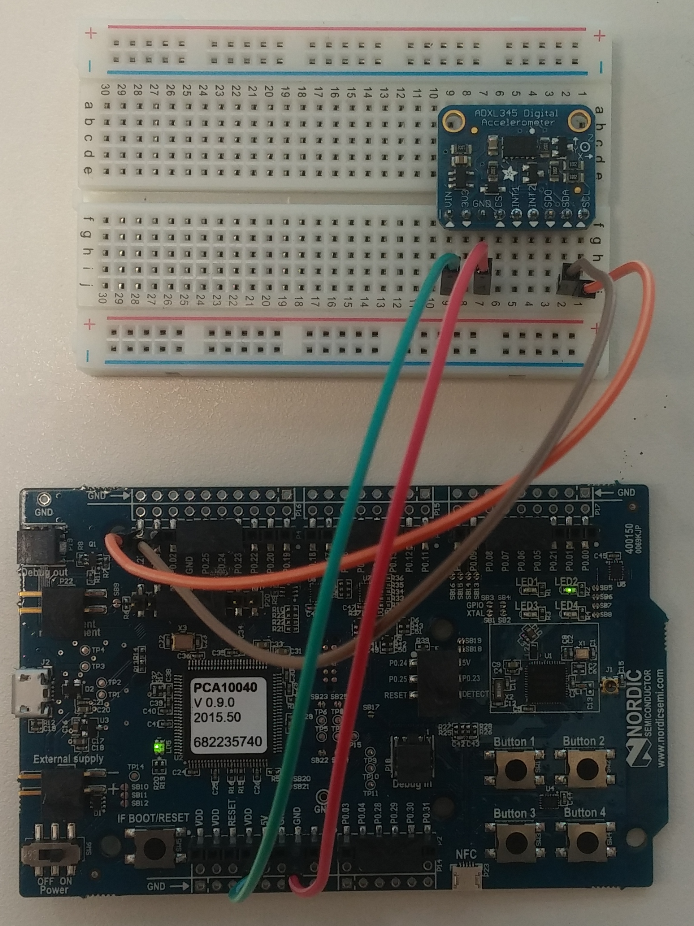
\includegraphics[scale=0.35]{nrf-adxl.png}    \caption{Connected nRF52 -- ADXL345}
    \label{fig:nrf-adxl345}
\end{figure}

After this is done it is possible to write to and read from the registers of the accelerometer over the two SDA and SCL cables. 


\subsection{Connection challenges}

Following instructions from a representative from Nordic Semiconductor, the bt0 interface was set up using the recommended \gls{ipv6} prefix: \textit{2001:bt8::1/64} in in the file \textit{etc/sysctrl.conf}, and after that trying to connect and test the connected devices using addresses on the form: 

\begin{verbatim}
ping6 2001:bt8::0211:22FF:FE33:4455
\end{verbatim}

This turned out not to work on the \gls{ipv6} network used on \gls{ntnu}, where the standard prefix is \textit{2001::1/64}, without the \textit{db8}. Both solutions should however work in other \gls{ipv6} networks. 

\subsection{bt8}

\todo{Descibe bt8-problem and devzone.nordicsemi.com and infocenter.nordicsemi.com}

\todo{Describe why I dropped the accelerometer}



\section{Nordic Semiconductor example code}

Nordic Semiconductor has provided several examples along with the nRF52-DK documentation, that can be used as a starting point when programming applications to the device. These files are written in the programming language \textit{C}. 

\subsection{\gls{coap}}

As a first step, the nRF52 needed to communicate with the Raspberry Pi. As explained in section 2.6, a good starting point for this is to use the \gls{coap} trasnport protocol, and the example of the use of this on the device. The \textit{CoAP Server} and \textit{CoAP Observer} was loaded into two different nRF52 devices, and both of them connected to the Raspberry Pi. Now \gls{radvd} had to be activated on the Pi, to be able to use this as a \textit{forwarding server}. 

\begin{figure}[ht]
    \centering
    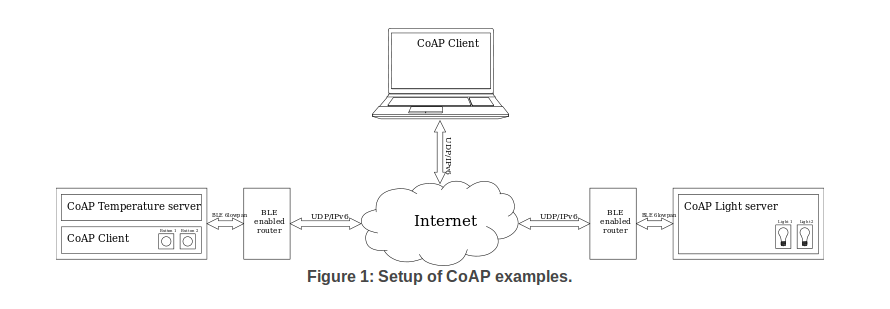
\includegraphics[scale=0.47]{CoAPExample.png}    
    \caption{CoAP Client-Server communication example}
    \label{fig:CoAPexample1}
\end{figure}
\todo{Remove "Figure 1" from image}

Figure \ref{fig:CoAPexample1} shows the initial CoAP example, by using two nRF52 devices, \gls{ble} over \gls{6lowpan} and a \gls{ble} enabled router (Raspberry Pi) on both ends in this case. As the figure \ref{fig:CoAPexample1} shows, the code example for the \gls{coap} client includes two different cases: 

\begin{itemize}
  \item In the fist case the \gls{coap} client acts as a client requesting services from the \gls{coap} server. Button 1 and 2 will control light 1 and 2 on the nRF52 server, which will send a conformation back if the light was changed or if something went wrong.
  \item In the second case the \gls{coap} server is excluded, but the \gls{coap} client works as a server that can handle requests from the router. In this case it is possible to use \textit{Copper} in a \textit{Firefox browser} on the Raspberry Pi to act as a client to request values from a simulated temperature sensor on the server. The server will  then send the current simulated temperature back, or tell if something went wrong. 
\end{itemize} 

Figure \ref{fig:CoAPexample1} shows the capture of packets using Wireshark. 

\begin{figure}[ht]
    \centering
    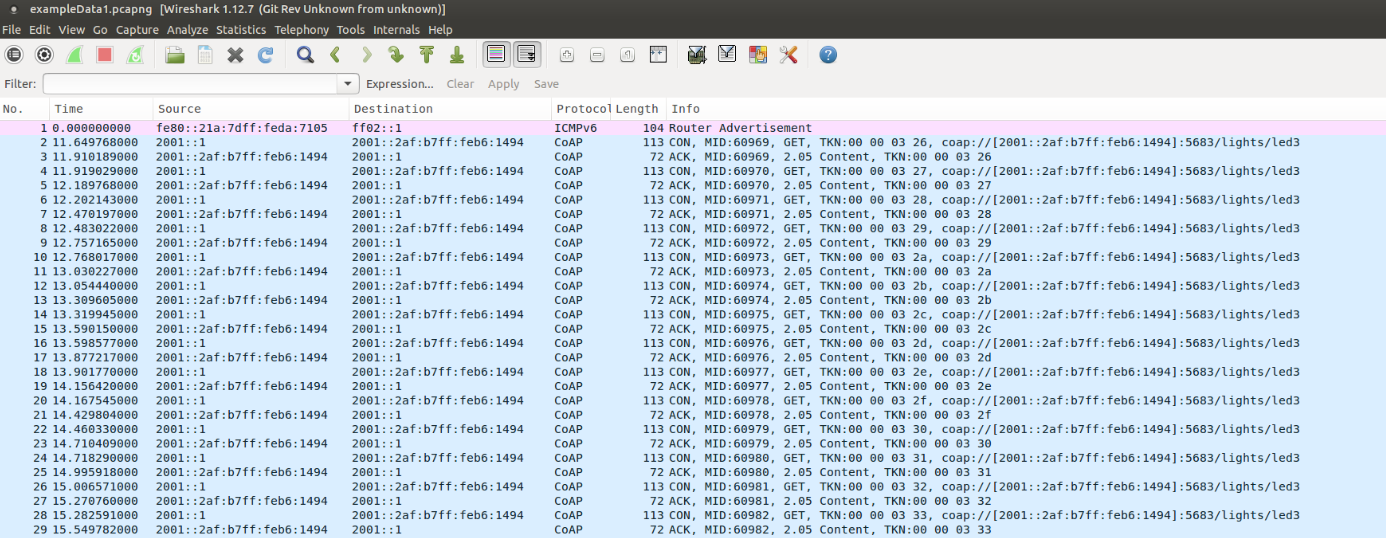
\includegraphics[scale=0.27]{CoapEx1captureCropped2.png}    
    \caption{CoAP Client-Server example Wireshark capture}
    \label{fig:CoAPexample1}
\end{figure}


This gives us the sequence diagram shown in Figure \ref{fig:seq1}. 

\begin{figure}[ht]
    \centering
    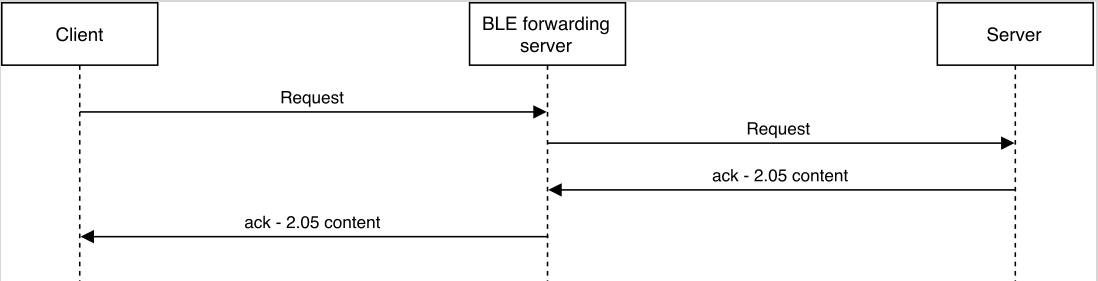
\includegraphics[scale=0.27]{seq1.png}    
    \caption{Sequence diagram CoAP Client-Server example}
    \label{fig:seq1}
\end{figure}

\todo{Create new sequence diagram}

This works fine, and by writing a Python script running on the \textit{Raspberry Pi} it is possible to request data by \textit{GET messages} as soon as the \textit{nRF52} is ready. However, as shown in figure \ref{fig:pingComparison} and figure \ref{fig:ping2}, the network transfer rate can vary a lot. The limitations in \gls{ble} and \gls{6lowpan} makes this much slower than a standard \gls{ipv6} connection, and the \textit{ping} \gls{rtt} varies from 100 ms all the way up to over 600 ms. As a comparison, to \textit{ping google.com} from the same Raspberry Pi using \gls{ipv6} takes on average 15 ms. A comparison of this is shown in figure \ref{fig:pingComparison}. This is therefore a clear limitation of sending rate in the system. Because of this, the maximum transfer rate achieved in the system using the standard \gls{coap} server example is one message every 200 ms. 

Using the standard \gls{coap}, described as \textit{CoAP CON} in this thesis, messages are sent with a "\gls{tcp} mindset". This means that every message sent by the client must receive an \gls {ack}. This is very stable, and ensures that every message gets to its destination, but it requires a lot of unnecessary computational power in the leaf node in systems where the importance of each message is not that high. The system is meant to be used with tools for analysing, and it is not essential that data needs to get to its destination right away. In these cases there is another alternative, known in this thesis as \textit{CoAP NON}. This is more like a "\textit{gls{udp} mindset}", where each packet does \textit{not} need an \gls{ack}. This halves the number of packages sent, saves a lot of the network as well as actions needed to be done by the nRF52 where power consumption is a huge issue. Therefore the \textit{\gls{coap} Observable} function looked very interesting, and will therefore be directly compared to \textit{standard gls{coap}} later in this thesis.   

%To improve this, the best solution is to either 

%This works fine, but in the case of the system built in this thesis there is no need to receive a confirmation for every single message.  It therefore makes sense to send messages in an \textit{\gls{udp} fashion}, where packages are being sent right away without acknowledgement. .   

\subsection{Observable \gls{coap}}

In the given Nordic example of a \gls{coap} observable server, the problem of unnecessary packets being sent can be resolved. Using this it is easy to set up a server that can be observed by either a nRF52 client or a \gls{ble} forwarding server. The observable end point sends a \textit{CON-ACK request} in a given time interval to assure that the observing client is still there. As long as this message is being responded the server will continue to send data without any requirements of an \gls{ack}. 

\begin{figure}[ht]
    \centering
    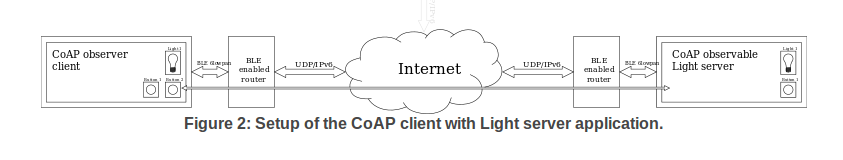
\includegraphics[scale=0.47]{CoAPObservalbFigure2.png}    
    \caption{CoAP Observable Server example}
    \label{fig:CoAPexample2}
\end{figure}
\todo{Remove "Figure 1" from image}



\todo{Create new sequence diagram for Observable as well}


\section{Getting acceleration values}

As soon as the sending of values is being handled in a good way, the next step is to read acceleration values from the ADXL345 accelerometer, which is connected to the NRF52 using the \gls{i2c} interface. 

Acceleration values can only be read from the ADXL345 if this has been correctly initialized at compile time. In order to do this, code to write to and read from the registers had to be added. The initializing process is described in the accelerometer data sheet \cite{adxlDataSheet}. In short, registers for \textit{data format control, initial power saving, interrupt enable control} and \textit{the offset of each axis} has to be written to in that order before the acceleration value from the different axes can be read.  

In the solution proposed in this thesis the acceleration values are being read as often as possible, limited by the processing power of the nRF52, and then stores in a simple dynamical char array before being sent and reset after one second. This turned out to be very time consuming and hard to solve in a good way, both because of problems with initializing the accelerometer correctly and making the nRF52 read and store the values fast enough to get proper data. The ideal solution would be to read at least 1000 values every second, to get a good starting point before analysing values. Neither the nRF52 or the ADXL345 turns out to be fast enough to do this in the implemented solution.  To not loose too much time on hardware problems, it was decided to focus more on analysing the data sent over the network communication with random generated data. 

Since the network connection between the nRF52 and Raspberry Pi was already stable, it was easy to generate random values of fixed length to send on the nRF52, and do measurements to calculate the optimal throughput between these two. The next chapter will therefore describe the data analysis of the data sent through this network in detail, and how to optimize the percentage of usable data being transported.  

\todo{Describe why not to gather acceleration values in this project}


\section{From Raspberry Pi to Network Computer or Server}

When running the Unix based \gls{os} Ubuntu Mate, the raspberry Pi can be used more or less as a regular computer. This has a pre-installed version of the most basic programs needed, for instance \textit{Mozilla Firefox Browser}, \textit{Pluma text editor} and \textit{Unix terminal}. This means that the user has several options on how to process data on this device: 

\begin{itemize}
  \item No computation: All data arrives as useful data, and can be posted directly to a web page or a server for storage
  \item No computation: Forward all data directly to a computer with more computational power
  \item Some computation: Analyse the data to find data that is not relevant to filter out
  \item Full computation: Do a full analyse of the data. The results can then be posted directly to a server or displayed on a web page. 
\end{itemize}

Which of these four options that is most relevant depends on the data, and how computational power is needed. It is possible to run the Raspberry Pi from a power bank, but this has not been tested in this project. When set up without a battery as power source, the Pi is the first node that could possibly do computations without having to take power limitations as a great concern. The main limitation is therefore computational power, while the main limitation may be battery power on the nRF52. It therefore makes sense to do some easy computation on this device. For instance, if this network is being used to measure vibrations, it is reasonable to assume about 1000 acceleration values every second, which represents a measuring rate of 1 kHz. It would then be perfectly reasonable to assume that the Pi could go through these values, and calculate whether or not the current acceleration value has breached a given threshold. This result can then be displayed directly on a web page or a connected monitor from the Pi. If however the system is to calculate \textit{patterns} in the acceleration values several values needs to be compared together. The need of complex algorithms to find these patterns is expected, before the results can be displayed. In this case it is reasonable to assume that the Pi would need additional computational power. The Pi can then be set up as a forwarding device, that forward data directly to a computer with more computational power. 



\renewcommand*{\bibname}{References}
\bibliographystyle{chicago} %alpha
\bibliography{main}

%% Uncomment the following if you have any appendix
 \appendix
 \addtocontents{toc}{%
  \protect\vspace{1em}% 
  \protect\noindent \bfseries \appendixtocname\protect\par
  \protect\vspace{-.5em}%
 }
 \renewcommand{\chaptername}{\appendixname}
%% include below possible appendices (chapters)


\end{document} 
